% Báo cáo đồ án cuối kỳ — Nhập môn Học máy
% Biên dịch: cd report && latexmk -xelatex main.tex
\documentclass[11pt,a4paper]{article}
\usepackage[a4paper,margin=2.3cm]{geometry}
\usepackage{fontspec}
\setmainfont{texgyretermes}[Extension=.otf,UprightFont=*-regular,BoldFont=*-bold,ItalicFont=*-italic,BoldItalicFont=*-bolditalic]
\setmonofont{texgyrecursor}[Extension=.otf,UprightFont=*-regular,BoldFont=*-bold,ItalicFont=*-italic,BoldItalicFont=*-bolditalic,Scale=0.95]
\usepackage[vietnamese]{babel}
\usepackage{amsmath,amssymb}
\usepackage{graphicx}
\usepackage{booktabs,tabularx,multirow,longtable}
\usepackage{xcolor}
\usepackage{caption,subcaption}
\usepackage{float}
\usepackage{enumitem}
\usepackage{tikz}
\usetikzlibrary{positioning,arrows.meta,fit,calc,shapes.misc}
\usepackage[hidelinks]{hyperref}
\usepackage{listings}
\lstset{basicstyle=\ttfamily\small,breaklines=true,frame=single,columns=fullflexible}
\setlist{itemsep=2pt,topsep=3pt}
\setlength{\emergencystretch}{3em}
\graphicspath{{../outputs/final/figures/}}
\newcommand{\tabdir}{../outputs/final/tables}
\newcommand{\code}[1]{\texttt{#1}}

\title{\textbf{Phát hiện ransomware trên chuỗi khối Bitcoin\\bằng mạng nơ-ron hồi tiếp (LSTM/GRU) và mạng tích chập (CNN)}\\[4pt]
\large Đồ án cuối kỳ — Nhập môn Học máy}
\author{Nhóm: [Họ tên thành viên — MSSV]}
\date{\today}

\begin{document}
\maketitle

\begin{abstract}
Đồ án áp dụng mạng nơ-ron hồi tiếp (LSTM, GRU) và mạng tích chập một chiều (CNN) cho bài toán phát hiện và phân loại ransomware
trên bộ dữ liệu BitcoinHeist (2,9 triệu dòng, 7 lớp, lớp \code{white} chiếm 98,6\%). Vì dữ liệu ở dạng bảng, chúng tôi so sánh hai
cách biểu diễn chuỗi: (A) coi 11 đặc trưng của một dòng là một chuỗi 11 bước, và (B) dựng chuỗi lịch sử thật của mỗi địa chỉ
qua các ngày (tối đa 16 lần xuất hiện), đánh giá trên cách chia theo địa chỉ để tránh rò rỉ. Hơn 40 cấu hình được thử nghiệm có
hệ thống (số tầng, số units, hai chiều, cách gộp chuỗi, BatchNorm, Dropout, kích thước kernel, pooling, learning rate, batch size,
độ dài lịch sử), các cấu hình chính chạy với 3 seed. Với biểu diễn A, RNN/CNN đạt macro F1 0,51--0,54 --- ngang MLP và thấp hơn
XGBoost (0,575): xếp đặc trưng thành chuỗi không tạo thêm thông tin. Với biểu diễn B, macro F1 tăng lên 0,72--0,74; mô hình
nơ-ron tốt nhất là CNN kernel 5 (0,742), vượt XGBoost cùng thông tin một dòng (0,565) nhưng vẫn thấp hơn XGBoost có đặc trưng lịch sử
tổng hợp (0,767). Phân tích chi tiết cho thấy RNN/CNN vượt XGBoost trên các địa chỉ có lịch sử dài ($\ge$6 lần xuất hiện) nhưng
thua trên các địa chỉ mới --- nhóm chiếm 90\% dữ liệu. Biểu diễn B dễ overfit hơn và được lợi rõ rệt từ BatchNorm + Dropout,
trong khi với biểu diễn A điều chuẩn thêm chỉ gây underfit.

\end{abstract}

\tableofcontents
\newpage

\section{Giới thiệu bài toán và mục tiêu}

Ransomware (mã độc tống tiền) mã hoá dữ liệu của nạn nhân và đòi tiền chuộc, thường được trả bằng Bitcoin. Vì mọi giao dịch Bitcoin
đều công khai trên chuỗi khối, ta có thể quan sát hành vi của các địa chỉ nhận tiền và đặt câu hỏi: \emph{chỉ từ các đặc trưng giao dịch
của một địa chỉ trong một ngày, có thể nhận ra địa chỉ đó là địa chỉ bình thường hay thuộc một họ ransomware cụ thể không?}

{\sloppy\paragraph{Bài toán.} Phân loại đa lớp (7 lớp): \code{white} (bình thường), 5 họ ransomware phổ biến nhất
(\code{paduaCryptoWall}, \code{montrealCryptoLocker}, \code{princetonCerber}, \code{princetonLocky}, \code{montrealCryptXXX})
và \code{otherRansom} (gộp 23 họ hiếm còn lại). Cách định nghĩa nhãn, đặc trưng và cách chia dữ liệu được giữ nguyên như bài giữa kỳ
(Bài~1) để các kết quả so sánh được với nhau.\par}

\paragraph{Mục tiêu đồ án.}
\begin{enumerate}
\item Xây dựng, huấn luyện và đánh giá mạng nơ-ron hồi tiếp (LSTM, GRU) và mạng tích chập 1 chiều (CNN Conv1D) cho bài toán trên.
\item Vì dữ liệu ở dạng bảng, đề xuất và so sánh \textbf{hai cách biểu diễn chuỗi}:
  (A) coi 11 đặc trưng của một dòng là một chuỗi;
  (B) dựng \emph{chuỗi lịch sử thật} của mỗi địa chỉ qua các ngày.
\item Thực nghiệm có hệ thống ($\approx$50 cấu hình, các cấu hình chính chạy 3 seed), so sánh với các mô hình nền (Logistic Regression, KNN, Random Forest,
  HistGradientBoosting, LightGBM, XGBoost, MLP), phân tích overfitting/underfitting và các lỗi dự đoán.
\item Đánh giá trung thực: chỉ ra khi nào RNN/CNN \emph{không} phải lựa chọn tốt nhất và vì sao.
\end{enumerate}

\section{Mô tả bộ dữ liệu}

\paragraph{Nguồn.} \emph{BitcoinHeistRansomwareAddressDataset} (UCI Machine Learning Repository; Akcora và cộng sự~[1]).
Dữ liệu gồm \textbf{2.916.697 dòng}, 10 cột, giai đoạn 2011--2018, \textbf{2.631.095 địa chỉ} khác nhau.
Mỗi dòng mô tả một địa chỉ Bitcoin trong một ngày (24 giờ), với các đặc trưng được tính từ đồ thị giao dịch (Bảng~\ref{tab:cols}).

\begin{table}[H]\centering\small
\caption{Các cột của bộ dữ liệu.}\label{tab:cols}
\begin{tabularx}{\linewidth}{llX}
\toprule
Cột & Kiểu & Ý nghĩa \\ \midrule
\code{address} & chuỗi & Địa chỉ Bitcoin (định danh, không dùng làm đặc trưng trực tiếp) \\
\code{year}, \code{day} & số nguyên & Năm (2011--2018) và ngày trong năm (1--365) \\
\code{length} & số & Độ dài chuỗi giao dịch dài nhất dẫn tới địa chỉ (0--144) \\
\code{weight} & số & Lượng ``đầu vào'' được gộp về địa chỉ \\
\code{count} & số & Số chuỗi giao dịch dẫn tới địa chỉ \\
\code{looped} & số & Số giao dịch tách ra rồi gộp lại (dấu hiệu ``trộn'' tiền) \\
\code{neighbors} & số & Số giao dịch có địa chỉ là đầu ra \\
\code{income} & số & Số satoshi nhận được ($1$~BTC $=10^8$ satoshi), từ $3\cdot10^7$ đến $5\cdot10^{13}$ \\
\code{label} & phân loại & \code{white} hoặc tên họ ransomware (28 họ) \\
\bottomrule
\end{tabularx}
\end{table}

\paragraph{Phân bố nhãn --- mất cân bằng nghiêm trọng.} Lớp \code{white} chiếm \textbf{98,58\%}; 6 lớp ransomware cộng lại chỉ có
41.413 dòng (1,42\%), lớp nhỏ nhất (\code{otherRansom}) chỉ 1.441 dòng (Bảng~\ref{tab:labels}). Vì vậy \emph{accuracy} gần như
vô nghĩa (đoán toàn \code{white} đã đạt 98,6\%); độ đo chính của đồ án là \textbf{macro F1} (trung bình F1 của 7 lớp, mỗi lớp
có trọng số như nhau), kèm F1 nhị phân ``ransomware hay không'', precision/recall từng lớp và ma trận nhầm lẫn.

\begin{table}[H]\centering\small
\caption{Phân bố 7 lớp và đặc điểm ``lặp lại'' của địa chỉ (tính trên toàn bộ dữ liệu).
\emph{Lần đầu}: tỉ lệ dòng mà địa chỉ chưa từng xuất hiện trước đó; \emph{trung vị số lần trước}: số lần địa chỉ đã xuất hiện ở các ngày trước.}
\label{tab:labels}
\begin{tabular}{lrrrrr}
\toprule
Lớp & Số dòng & Tỉ lệ (\%) & Số địa chỉ & Lần đầu (\%) & Trung vị số lần trước \\ \midrule
\code{white} & 2.875.284 & 98,580 & 2.610.246 & 90,8 & 0 \\
\code{paduaCryptoWall} & 12.390 & 0,425 & 1.894 & 15,3 & 5 \\
\code{montrealCryptoLocker} & 9.315 & 0,319 & 1.509 & 16,2 & 13 \\
\code{princetonCerber} & 9.223 & 0,316 & 9.177 & 99,5 & 0 \\
\code{princetonLocky} & 6.625 & 0,227 & 6.584 & 99,4 & 0 \\
\code{montrealCryptXXX} & 2.419 & 0,083 & 1.354 & 56,0 & 0 \\
\code{otherRansom} & 1.441 & 0,049 & 331 & 23,0 & 6 \\
\bottomrule
\end{tabular}
\end{table}

\paragraph{Các đặc điểm quan trọng.}
\begin{itemize}
\item \textbf{Đặc trưng lệch rất mạnh}: \code{income} trải dài 6 bậc độ lớn, \code{count}/\code{looped} có trung vị 1/0 nhưng
  tối đa $\approx 14.500$ $\Rightarrow$ cần biến đổi $\log(1+x)$ trước khi chuẩn hoá.
\item \textbf{\code{white} được lấy mẫu cố định 1.000 dòng/ngày} (365.000 dòng mỗi năm), còn ransomware thì lấy đủ. Tỉ lệ ransomware
  thay đổi mạnh theo năm (0,001\% năm 2018 đến 4,1\% năm 2016) nên năm/tháng là thông tin hữu ích.
\item \textbf{Địa chỉ có thể xuất hiện nhiều ngày} (Bảng~\ref{tab:labels}). Đây là điểm mấu chốt cho biểu diễn chuỗi B:
  \code{CryptoLocker}, \code{CryptoWall}, \code{otherRansom} \emph{tái sử dụng} địa chỉ rất nhiều (chỉ 15--23\% dòng là lần đầu),
  trong khi \code{Cerber}, \code{Locky} gần như luôn dùng địa chỉ mới (99,5\%), giống \code{white} (90,8\%).
  Không có địa chỉ nào mang hai nhãn khác nhau.
\item Hệ quả: nếu chia train/test ngẫu nhiên theo dòng, \textbf{cùng một địa chỉ ransomware có thể nằm ở cả train và test}
  (55\% dòng ransomware trong test có địa chỉ đã xuất hiện trong train). Biểu diễn B vì vậy bắt buộc phải \emph{chia theo địa chỉ}.
\end{itemize}

\paragraph{Dạng bài toán.} Phân loại có giám sát, đa lớp, dữ liệu bảng, mất cân bằng nặng.
Dữ liệu \emph{không} phải ảnh, văn bản hay chuỗi thời gian ``tự nhiên'' --- mục~\ref{sec:repr} trình bày cách chuyển đổi để dùng RNN và CNN.

\section{Tiền xử lý và chuẩn bị dữ liệu}\label{sec:prep}

\paragraph{Làm sạch.} Dữ liệu không có giá trị thiếu và không có dòng trùng lặp hoàn toàn; không cần điền khuyết.
Cột \code{address} chỉ dùng để nhóm (dựng lịch sử, chia dữ liệu theo địa chỉ), không đưa trực tiếp vào mô hình.

\paragraph{Định nghĩa nhãn.} 5 họ ransomware nhiều mẫu nhất giữ nguyên tên, 23 họ còn lại gộp thành \code{otherRansom}
(nhiều họ chỉ có 1--60 dòng, không thể học riêng) $\Rightarrow$ 7 lớp.

\paragraph{Xây dựng đặc trưng (giống Bài 1).}
\begin{itemize}
\item 6 đặc trưng gốc: \code{length, weight, count, looped, neighbors, income}.
\item 5 đặc trưng mới: \code{income\_tz} (số chữ số 0 ở cuối \code{income} --- độ ``tròn'' của số tiền, tiền chuộc thường là số tròn),
  \code{income\_per\_count}, \code{income\_per\_neighbor}, \code{weight\_per\_count}, \code{looped\_ratio}.
\item Thời gian: \code{year}, \code{month}, \code{weekday} (tính từ \code{year} + \code{day}), mã hoá \textbf{one-hot}
  (8 + 12 + 7 = 27 chiều).
\end{itemize}

\paragraph{Chuẩn hoá.} 11 đặc trưng số được biến đổi $x \mapsto \log(1+x)$ rồi chuẩn hoá $z=(x-\mu)/\sigma$, với $\mu,\sigma$
\textbf{chỉ tính trên tập train} (tránh rò rỉ thông tin từ validation/test).

\paragraph{Chia dữ liệu.} Tỉ lệ train/validation/test = 64/16/20, cố định \code{random\_state=42}, mọi mô hình trong cùng một
nhóm thí nghiệm dùng \emph{chung} một cách chia:
\begin{itemize}
\item \textbf{Chia ngẫu nhiên phân tầng theo nhãn} (dùng cho biểu diễn A, giống hệt Bài 1):
  train 1.866.685 / validation 466.672 / test 583.340 dòng (test có 8.283 dòng ransomware).
\item \textbf{Chia theo địa chỉ} (\code{GroupShuffleSplit}; dùng cho biểu diễn B): mọi dòng của một địa chỉ nằm trọn trong
  một tập. Train 1.867.045 / validation 466.842 / test 582.810 dòng (7.911 dòng ransomware trong test).
  Đã kiểm tra: không có địa chỉ nào xuất hiện ở cả train và test.
\end{itemize}

\paragraph{Xử lý mất cân bằng (giống Bài 1).}
\begin{enumerate}
\item \textbf{Undersampling tập train}: giữ ngẫu nhiên 100.000 dòng \code{white} + toàn bộ dòng ransomware
  $\Rightarrow$ khoảng 126.500 dòng (ransomware chiếm $\approx$21\%). Bài 1 đã chứng minh mức 100k cho macro F1 tốt nhất.
\item \textbf{Hiệu chỉnh trọng số lớp sau huấn luyện}: mô hình học trên phân bố đã cân bằng nên dự đoán ``nghiêng'' về ransomware.
  Trên tập \emph{validation} (phân bố thật), ta tìm vector $w\in\mathbb{R}^7$ (dò lưới theo từng lớp, 3 vòng) sao cho
  $\hat y=\arg\max_k p_k w_k$ có macro F1 cao nhất; $w$ sau đó được giữ cố định khi đánh giá test.
\end{enumerate}
Tập validation còn được dùng ở dạng \textbf{val\_us} --- undersample \code{white} cùng tỉ lệ với tập train (31.626 dòng) ---
để đường cong loss/F1 của train và validation \emph{so sánh được với nhau} và để early stopping.
\textbf{Tập test chỉ được dùng một lần}, sau khi mô hình, epoch tốt nhất và trọng số $w$ đã được chọn hoàn toàn trên train/validation.

\section{Phương pháp và kiến trúc mô hình}

\subsection{Biểu diễn dữ liệu thành chuỗi}\label{sec:repr}

Mỗi dòng của BitcoinHeist là một vector đặc trưng, không có cấu trúc chuỗi sẵn có. Đồ án thử hai cách chuyển đổi (Hình~\ref{fig:repr}).

\begin{figure}[H]\centering
\begin{tikzpicture}[font=\small, tok/.style={draw,rounded corners=1pt,minimum width=0.95cm,minimum height=0.55cm,fill=blue!8},
  hstep/.style={draw,rounded corners=1pt,minimum width=1.25cm,minimum height=0.55cm,fill=orange!12},
  pad/.style={draw,dashed,rounded corners=1pt,minimum width=1.25cm,minimum height=0.55cm,fill=gray!8}]
\node[anchor=west] at (-0.6,1.0) {\textbf{(A) Feature-as-sequence}: 1 dòng $\to$ chuỗi 11 bước, bước $i$ = đặc trưng thứ $i$};
\foreach \n [count=\i from 0] in {length,weight,count,looped,neigh.,income,inc\_tz,inc/cnt,inc/nb,w/cnt,loop/cnt}
  \node[tok] (a\i) at (\i*1.08,0) {\scriptsize \n};
\node[below=0.15cm of a5] {\scriptsize $x_i \;\mapsto\; x_i\mathbf{W}_i+\mathbf{b}_i\in\mathbb{R}^{16}$ \quad (thứ tự đặc trưng do ta đặt, không mang nghĩa thời gian)};
\node[anchor=west] at (-0.6,-1.55) {\textbf{(B) Address history}: dòng hiện tại + tối đa $L-1$ lần xuất hiện \emph{trước đó} của cùng địa chỉ};
\node[hstep] (b0) at (0.1,-2.5) {\scriptsize ngày $t_1$};
\node[hstep,right=0.15cm of b0] (b1) {\scriptsize ngày $t_2$};
\node[hstep,right=0.15cm of b1] (b2) {\scriptsize $\cdots$};
\node[hstep,right=0.15cm of b2,fill=red!15,thick] (b3) {\scriptsize hôm nay};
\node[pad,right=0.15cm of b3] (b4) {\scriptsize đệm};
\node[pad,right=0.15cm of b4] (b5) {\scriptsize đệm};
\node[right=0.2cm of b5,align=left] {\scriptsize mỗi bước: 11 đặc trưng\\\scriptsize + cờ ``lần đầu'' + $\log(1+\Delta\text{ngày})$};
\draw[-{Latex}] (b0.south west) ++(0,-0.15) -- ($(b3.south east)+(0,-0.15)$) node[midway,below] {\scriptsize thời gian (chỉ quá khứ, không nhìn tương lai)};
\end{tikzpicture}
\caption{Hai cách biểu diễn một dòng dữ liệu bảng thành chuỗi để đưa vào RNN/CNN.}\label{fig:repr}
\end{figure}

\paragraph{Biểu diễn A --- ``feature-as-sequence''.} 11 đặc trưng số (đã chuẩn hoá) được xem là chuỗi độ dài cố định 11.
Mỗi giá trị vô hướng $x_i$ được ``nhúng'' thành vector $\mathbf{e}_i=x_i\mathbf{W}_i+\mathbf{b}_i\in\mathbb{R}^{16}$, trong đó
$\mathbf{W}_i,\mathbf{b}_i$ là tham số \emph{riêng} của từng đặc trưng (\emph{feature tokenizer}~[8]) --- nhờ đó mô hình biết
bước $i$ là đặc trưng nào. Không có chuỗi dài ngắn khác nhau nên không cần đệm. 27 chiều one-hot thời gian không đưa vào chuỗi
mà được \emph{ghép vào trước lớp phân loại}. \textbf{Hạn chế}: thứ tự đặc trưng là tuỳ ý, không có ``thời gian'' hay ``vị trí''
thật; giả thiết cục bộ của CNN (đặc trưng kề nhau liên quan nhau) và giả thiết tuần tự của RNN chỉ đúng một phần (các đặc trưng
tỉ lệ được đặt cạnh đặc trưng gốc tương ứng). Do đó ta \emph{không kỳ vọng} RNN/CNN vượt mô hình cây trên biểu diễn này.

\paragraph{Biểu diễn B --- ``address history''.} Với mỗi dòng (địa chỉ $a$, ngày $t$), lấy tối đa $L=16$ lần xuất hiện gần nhất
của $a$ tại các ngày $\le t$, sắp theo thời gian, bước cuối là chính dòng hiện tại. Mỗi bước là vector 13 chiều
(11 đặc trưng + cờ ``lần đầu xuất hiện'' + $\log(1+\text{số ngày từ lần trước})$), chiếu tuyến tính sang $\mathbb{R}^{32}$.
\textbf{Chuỗi có độ dài khác nhau} (1--16): đệm 0 ở cuối, kèm mặt nạ (mask); RNN dùng \code{pack\_padded\_sequence} để bỏ qua
phần đệm, CNN nhân mặt nạ trước mỗi lớp tích chập và dùng pooling có mặt nạ. Đây là chuỗi thời gian \emph{thật}, chỉ dùng thông
tin quá khứ (có thể triển khai thực tế: khi một địa chỉ nhận tiền hôm nay, ta đã biết lịch sử của nó). Phải chia dữ liệu theo địa
chỉ để mô hình không ``nhớ'' địa chỉ đã thấy khi train.

\subsection{Mô hình RNN (LSTM / GRU)}

\begin{figure}[H]\centering
\resizebox{\linewidth}{!}{%
\begin{tikzpicture}[font=\small,node distance=0.45cm, box/.style={draw,rounded corners=2pt,align=center,minimum height=0.8cm,fill=#1}, box/.default=white]
\node[box=gray!10] (in) {Chuỗi đầu vào\\ $T\times$ đặc trưng};
\node[box=blue!8,right=of in] (emb) {Tokenizer (A) / \\ Linear (B)\\ $\to T\times d$};
\node[box=green!10,right=of emb] (rnn) {LSTM / GRU\\ $n$ tầng $\times h$ units\\ (Bi-)};
\node[box=green!5,right=of rnn] (pool) {Biểu diễn chuỗi:\\ hidden cuối /\\ mean / attention};
\node[box=orange!10,right=of pool] (cat) {Ghép one-hot\\ thời gian (27)};
\node[box=red!8,right=of cat] (head) {Dense 64, ReLU\\ Dropout\\ Dense 7, softmax};
\foreach \a/\b in {in/emb,emb/rnn,rnn/pool,pool/cat,cat/head} \draw[-{Latex}] (\a) -- (\b);
\end{tikzpicture}}
\caption{Kiến trúc tổng quát của mô hình RNN.}\label{fig:rnn}
\end{figure}

\begin{itemize}
\item \textbf{Lớp hồi tiếp}: LSTM (cổng quên/vào/ra + ô nhớ $c_t$) hoặc GRU (cổng cập nhật/đặt lại, không có ô nhớ riêng, ít
  tham số hơn $\approx$25\%). Cấu hình gốc: 1 tầng, 64 hidden units, một chiều. Các biến thể: 2 tầng, 128 units, hai chiều
  (Bidirectional), không dropout.
\item \textbf{Biểu diễn cuối của chuỗi}: hidden state cuối của tầng trên cùng (mặc định; với Bi-RNN ghép trạng thái cuối của hai
  chiều), trung bình (mean pooling) trên các bước thật, hoặc attention đơn giản $\alpha_t=\mathrm{softmax}_t(\mathbf{v}^\top
  \mathbf{h}_t)$, $\mathbf{z}=\sum_t\alpha_t\mathbf{h}_t$. Ở biểu diễn B, nhờ \code{pack\_padded\_sequence} hidden state cuối chính là
  trạng thái tại ngày hiện tại.
\item \textbf{Dropout}: 0,2 ở lớp Dense cuối và \emph{giữa các tầng} RNN khi có 2 tầng. \emph{Không dùng recurrent dropout}
  (dropout trên kết nối hồi tiếp) vì cài đặt cuDNN của PyTorch không hỗ trợ; với 1 tầng và chuỗi ngắn, dropout ở đầu ra là đủ.
\item \textbf{Đầu ra}: Dense 7 + softmax; hàm mất mát cross-entropy.
\end{itemize}
Chọn \textbf{cả LSTM và GRU} để so sánh kiến trúc, tốc độ và kết quả (mục~\ref{sec:results}).

\subsection{Mô hình CNN (Conv1D)}

\begin{figure}[H]\centering
\resizebox{\linewidth}{!}{%
\begin{tikzpicture}[font=\small,node distance=0.4cm, box/.style={draw,rounded corners=2pt,align=center,minimum height=0.8cm,fill=#1}, box/.default=white]
\node[box=gray!10] (in) {Chuỗi\\ $T\times d$};
\node[box=blue!8,right=of in] (c1) {Conv1D 32, k3\\ (BN) ReLU\\ (Dropout)};
\node[box=blue!4,right=of c1] (p1) {MaxPool 2\\ $T\to\lceil T/2\rceil$};
\node[box=blue!8,right=of p1] (c2) {Conv1D 64, k3\\ (BN) ReLU\\ (Dropout)};
\node[box=blue!4,right=of c2] (p2) {MaxPool 2};
\node[box=green!8,right=of p2] (fl) {Flatten /\\ Global Avg/Max\\ Pooling};
\node[box=red!8,right=of fl] (head) {+ one-hot 27\\ Dense 64, ReLU\\ Dense 7, softmax};
\foreach \a/\b in {in/c1,c1/p1,p1/c2,c2/p2,p2/fl,fl/head} \draw[-{Latex}] (\a) -- (\b);
\end{tikzpicture}}
\caption{Kiến trúc tổng quát của mô hình CNN 1 chiều.}\label{fig:cnn}
\end{figure}

\begin{itemize}
\item \textbf{Loại}: Conv1D (trượt dọc trục chuỗi, mỗi bước có $d$ kênh = chiều embedding). Conv2D không phù hợp vì dữ liệu không có
  cấu trúc 2 chiều.
\item \textbf{Lớp tích chập}: 2 lớp (32 và 64 filters) mặc định; biến thể 3 lớp (32-64-128), rộng (64-128), kernel 3 hoặc 5,
  padding ``same''. Mỗi filter là một bộ phát hiện mẫu \emph{cục bộ} trên $k$ bước liên tiếp, dùng chung trọng số ở mọi vị trí
  (chia sẻ tham số) --- với biểu diễn A là tổ hợp của $k$ đặc trưng kề nhau, với B là mẫu hành vi trong $k$ lần xuất hiện liên tiếp.
\item \textbf{Pooling}: MaxPooling (biến thể AveragePooling) kích thước 2 sau mỗi lớp khi chuỗi còn dài $\ge 4$:
  giảm một nửa độ dài $\Rightarrow$ giảm số tham số của lớp Dense phía sau và tính toán, đồng thời giúp đặc trưng ít nhạy với
  dịch chuyển nhỏ (bất biến cục bộ).
\item \textbf{Batch Normalization} và \textbf{Dropout} (0,3): bật/tắt để so sánh CNN đơn giản với CNN có điều chuẩn.
\item \textbf{Chuyển sang lớp phân loại}: \emph{Flatten} (giữ thông tin vị trí --- hợp với A vì mỗi vị trí là một đặc trưng cố định)
  hoặc \emph{Global Average/Max Pooling} (bất biến độ dài --- bắt buộc với B vì chuỗi dài ngắn khác nhau).
\item \textbf{Phần fully connected}: ghép one-hot thời gian $\to$ Dense 64 ReLU $\to$ Dropout $\to$ Dense 7 softmax.
\end{itemize}

\subsection{Mô hình nền (baseline)}
\begin{itemize}
\item Từ Bài 1 (cùng cách chia ngẫu nhiên, cùng tiền xử lý): Logistic Regression, KNN, Random Forest, HistGradientBoosting,
  LightGBM, XGBoost và Ensemble.
\item \textbf{MLP} (2 tầng ẩn 128 units, ReLU, Dropout 0,2): cùng đặc trưng nhưng \emph{không} coi là chuỗi --- dùng để tách bạch
  lợi ích của ``cấu trúc chuỗi'' khỏi lợi ích của ``mạng nơ-ron''.
\item \textbf{XGBoost trên cách chia theo địa chỉ} với 3 mức thông tin lịch sử: chỉ dòng hiện tại (\code{XGB\_current}); thêm
  số lần đã xuất hiện + khoảng cách ngày (\code{XGB\_count}); thêm trung bình/max của 11 đặc trưng trên 15 lần xuất hiện trước
  (\code{XGB\_hist}). Đây là đối thủ ``dạng bảng'' công bằng của biểu diễn B.
\end{itemize}

\section{Thiết lập thực nghiệm}\label{sec:setup}

\paragraph{Môi trường.} PyTorch 2.11 (CUDA 12.8), GPU NVIDIA RTX PRO 4000 Blackwell 24\,GB (máy chủ Trainbox, Windows), Python 3.12.
Toàn bộ dữ liệu của tập train/validation/test được đặt sẵn trên GPU; batch được cắt theo chỉ số dòng. Mã nguồn: thư mục \code{final/}
(\code{data.py}, \code{models.py}, \code{configs.py}, \code{train.py}, \code{baselines.py}, \code{report.py}) và notebook
\code{final\_project.ipynb}.

\paragraph{Huấn luyện (chung cho mọi mạng nơ-ron).}
\begin{itemize}
\item Hàm mất mát: \textbf{cross-entropy} trên đầu ra softmax 7 lớp. Thuật toán tối ưu: \textbf{Adam}, learning rate $10^{-3}$
  (biến thể $3\cdot10^{-4}$), batch size 512 (biến thể 2048), cắt gradient theo chuẩn $\le 1$.
\item Tối đa 100 epoch, \textbf{early stopping} theo macro F1 trên \code{val\_us} với patience 10; giữ lại trọng số của epoch tốt nhất.
\item Sau huấn luyện: tìm trọng số lớp $w$ trên toàn bộ validation $\to$ đánh giá test bằng $\arg\max(p\cdot w)$ (mục~\ref{sec:prep}).
\item Seed 42 cho mọi cấu hình; các cấu hình chính được chạy lại với seed 43, 44 để ước lượng độ dao động
  (báo cáo trung bình $\pm$ độ lệch chuẩn). Thay đổi seed chỉ thay đổi khởi tạo trọng số và thứ tự batch --- tập dữ liệu giữ nguyên.
\end{itemize}

\paragraph{Thiết kế thực nghiệm.} Mỗi lần chỉ thay đổi \emph{một} yếu tố so với cấu hình gốc của nhóm để thấy rõ ảnh hưởng:
\begin{itemize}
\item \textbf{RNN} (gốc: LSTM 1 tầng $\times$ 64 units, hidden state cuối, dropout 0,2): LSTM $\leftrightarrow$ GRU; 1 $\leftrightarrow$ 2 tầng;
  64 $\leftrightarrow$ 128 units; một chiều $\leftrightarrow$ hai chiều; hidden cuối $\leftrightarrow$ mean $\leftrightarrow$ attention;
  dropout 0,2 $\leftrightarrow$ 0; learning rate; batch size; độ dài lịch sử $L\in\{1,4,16,32\}$ (biểu diễn B).
\item \textbf{CNN} (gốc A: Conv 32-64, kernel 3, MaxPool, Flatten, không BN/Dropout): + BN; + Dropout; + BN + Dropout;
  Flatten $\leftrightarrow$ GAP; 2 $\leftrightarrow$ 3 lớp; số filters; kernel 3 $\leftrightarrow$ 5; Max $\leftrightarrow$ Average pooling;
  learning rate; batch size. Biểu diễn B dùng GAP (hoặc Global Max) vì chuỗi có độ dài thay đổi.
\item \textbf{Đối chứng}: MLP (không coi là chuỗi); \code{B\_gru\_L1} (biểu diễn B nhưng chỉ 1 bước = không có lịch sử);
  các biến thể \code{\_cnt} thêm đặc trưng đếm vào đầu vào phụ để so sánh công bằng với \code{XGB\_count}.
\end{itemize}

\paragraph{Độ đo.} Macro F1 (chính), F1 nhị phân ransomware/white, accuracy, precision/recall/F1 có trọng số và macro, F1 từng lớp,
ma trận nhầm lẫn; thời gian huấn luyện (tổng và trung bình mỗi epoch) và số tham số.

\section{Kết quả thực nghiệm}\label{sec:results}

Tất cả số liệu là trên \textbf{tập test}, sau khi chọn epoch (early stopping trên \code{val\_us}) và trọng số lớp $w$ (trên
validation). Với cấu hình chạy 3 seed (42, 43, 44), bảng ghi trung bình $\pm$ độ lệch chuẩn của macro F1; các cột khác lấy
trung bình. Cột ``Ep.'' là \emph{epoch tốt nhất / số epoch đã chạy} (early stopping dừng sau 10 epoch không cải thiện).

\subsection{Biểu diễn A --- mỗi đặc trưng là một bước (chia ngẫu nhiên, so sánh với Bài 1)}

\input{\tabdir/tab_A_rnn}
\input{\tabdir/tab_A_cnn}

\begin{figure}[H]\centering
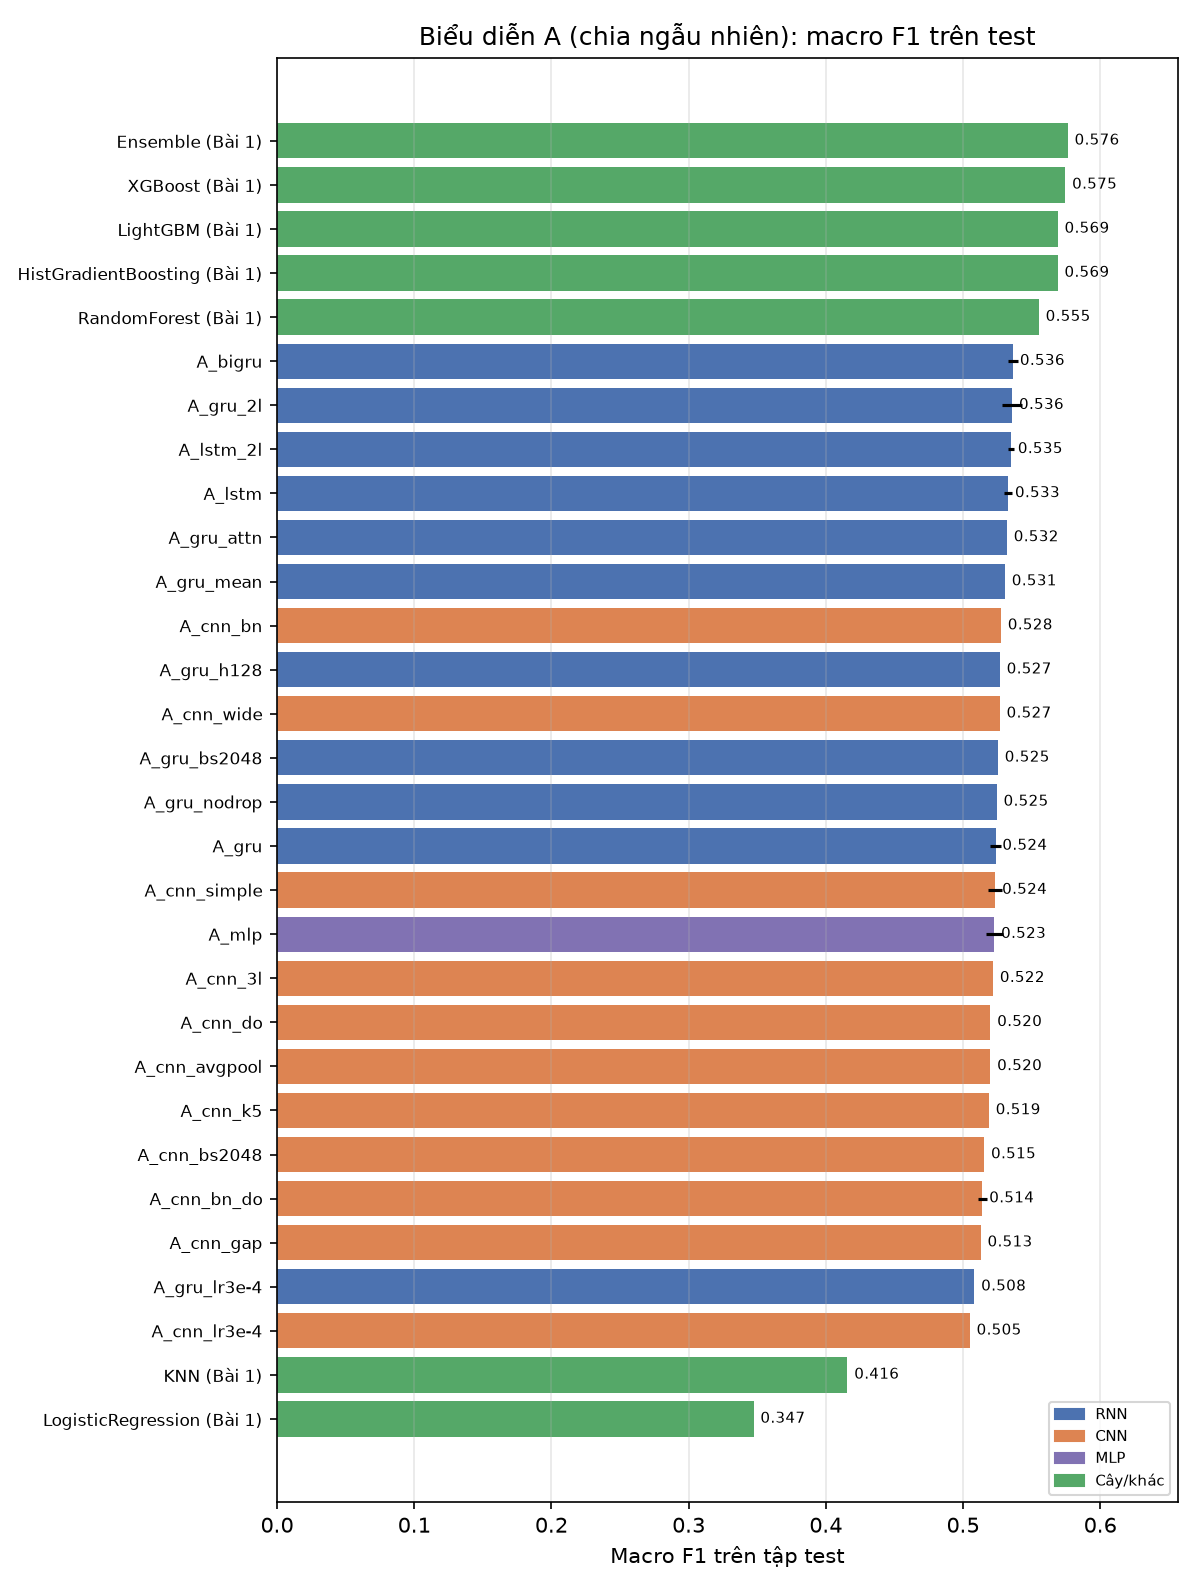
\includegraphics[width=0.82\linewidth]{bars_A.png}
\caption{Biểu diễn A: macro F1 trên test của mọi cấu hình RNN/CNN/MLP và các mô hình của Bài 1 (cùng cách chia, cùng tiền xử lý).
Vạch đen: độ lệch chuẩn qua 3 seed.}\label{fig:bars_A}
\end{figure}

\paragraph{Nhận xét.}
\begin{itemize}
\item Mọi cấu hình RNN nằm trong khoảng macro F1 0,51--0,54, CNN trong khoảng 0,50--0,53. Tốt nhất là \code{A\_bigru}, \code{A\_gru\_2l}, \code{A\_lstm\_2l}
  ($\approx$0,535--0,537) và \code{A\_cnn\_bn} (0,528). Độ lệch chuẩn giữa các seed là 0,002--0,007, nên phần lớn
  khác biệt giữa các biến thể RNN (LSTM/GRU, 1/2 tầng, một/hai chiều, last/mean/attention) \textbf{không có ý nghĩa thống kê}.
\item \textbf{MLP} (không coi dữ liệu là chuỗi) đạt $\approx$0,52 --- ngang RNN/CNN. Việc ``xếp 11 đặc trưng thành chuỗi''
  không mang lại thông tin mới: thứ tự các đặc trưng là tuỳ ý, phép tích chập trên ``đặc trưng kề nhau'' và trạng thái ẩn ``truyền
  từ đặc trưng này sang đặc trưng kia'' không có ý nghĩa vật lý. Đúng như đề bài cảnh báo ở mục 14.
\item \textbf{XGBoost của Bài 1 (0,575) vẫn tốt hơn mọi mạng nơ-ron trên biểu diễn A} (kể cả Random Forest 0,555 cũng hơn).
  Điều này khớp với kết quả đã biết: với dữ liệu bảng có đặc trưng lệch phân phối mạnh và quan hệ dạng ngưỡng, mô hình cây vẫn mạnh
  hơn mạng nơ-ron [9]. Mạng nơ-ron chỉ vượt Logistic Regression (0,347) và KNN (0,416).
\item Learning rate nhỏ ($3\cdot10^{-4}$) cho kết quả kém nhất ở cả RNN và CNN (underfit, xem mục~\ref{sec:analysis});
  batch 2048 làm số bước cập nhật mỗi epoch giảm 4 lần, mô hình GRU chạm giới hạn 100 epoch trước khi hội tụ.
\item Với CNN, thêm BatchNorm giúp hội tụ nhanh và cho kết quả tốt nhất; Dropout (0,3) và GAP làm giảm kết quả --- mô hình
  $\approx$23 nghìn tham số trên 126 nghìn mẫu không thừa năng lực, điều chuẩn thêm chỉ làm nó underfit. Flatten tốt hơn GAP vì
  ở biểu diễn A \emph{vị trí} chính là \emph{danh tính của đặc trưng}.
\end{itemize}

\subsection{Biểu diễn B --- lịch sử của địa chỉ (chia theo địa chỉ)}

\input{\tabdir/tab_B}
\input{\tabdir/tab_group_other}

\begin{figure}[H]\centering
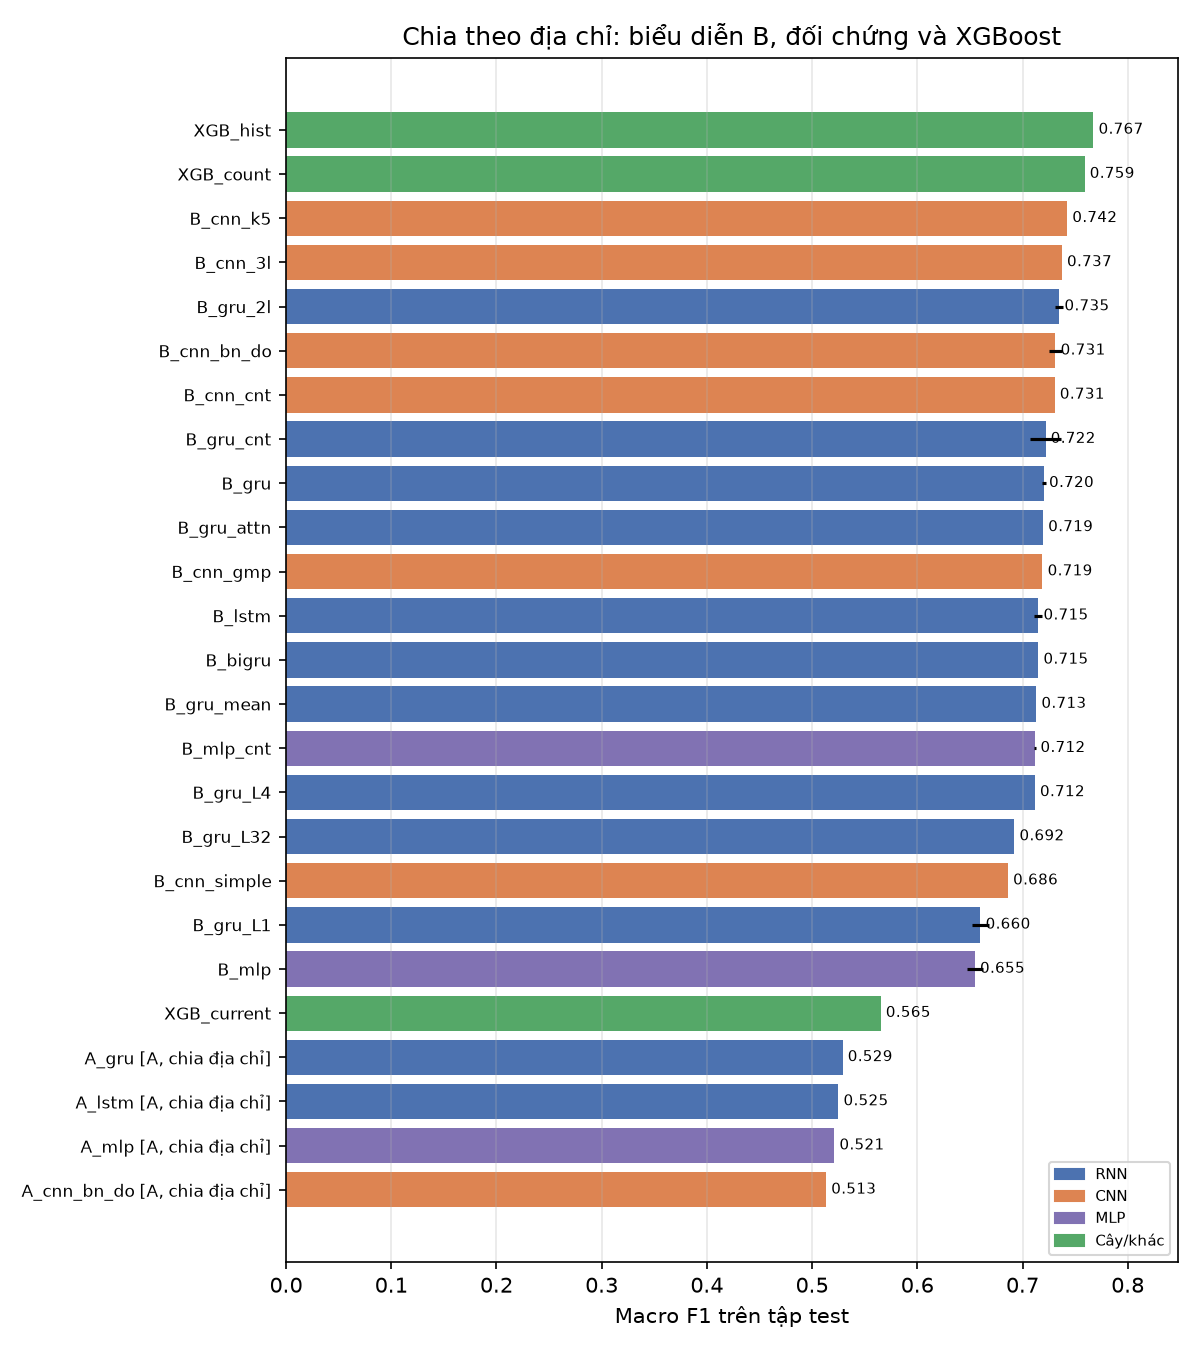
\includegraphics[width=0.78\linewidth]{bars_B.png}
\caption{Cùng cách chia theo địa chỉ: biểu diễn B, các biến thể đối chứng, XGBoost với 3 mức thông tin lịch sử và biểu diễn A.}
\label{fig:bars_B}
\end{figure}

\paragraph{Nhận xét.}
\begin{itemize}
\item \textbf{Biểu diễn B tăng macro F1 từ $\approx$0,53 lên $\approx$0,72--0,74} so với chính các mô hình đó trên biểu diễn A
  (cùng cách chia theo địa chỉ, Bảng~\ref{tab:group_other}). Đây là thông tin thật sự mới mà một dòng đơn lẻ không có: một địa
  chỉ ransomware (CryptoLocker, CryptoWall) nhận tiền nhiều ngày liên tiếp với mẫu hành vi lặp lại.
\item \textbf{Mô hình nơ-ron tốt nhất là CNN}: \code{B\_cnn\_k5} (0,742) và \code{B\_cnn\_3l} (0,737); RNN tốt nhất là
  \code{B\_gru\_2l} (0,735 $\pm$ 0,004). Trên B, \emph{tăng trường nhìn} (kernel 5, thêm tầng) có ích vì chuỗi dài hơn
  (tới 16 bước) và mẫu hành vi trải dài nhiều lần xuất hiện.
\item \textbf{Phần lợi ích do chuỗi mang lại}: \code{B\_gru\_L1} (chỉ bước hiện tại, nhưng có cờ ``lần đầu'' và khoảng cách ngày)
  đạt 0,660; L=4 đạt 0,712 và L=16 đạt 0,720. So với biểu diễn A trên cùng cách chia ($\approx$0,53), riêng việc \emph{biết địa chỉ
  từng xuất hiện} đã cho +0,13, và việc \emph{nhìn thấy nội dung các lần xuất hiện trước} cho thêm +0,06--0,08. L=32 không tốt hơn (0,692; dừng sớm ở epoch 26):
  địa chỉ có $>$16 lần xuất hiện rất ít, phần đệm dài chỉ thêm nhiễu.
\item \textbf{Đối chứng công bằng với XGBoost}: XGBoost chỉ dùng dòng hiện tại đạt 0,565; thêm 3 đặc trưng đếm
  (số lần đã xuất hiện, cờ lần đầu, khoảng cách ngày) đạt 0,759; thêm trung bình/max lịch sử đạt \textbf{0,767 --- tốt nhất toàn
  bộ đồ án}. Khi được cho cùng thông tin lịch sử dưới dạng đặc trưng tổng hợp thủ công, mô hình cây vẫn hơn RNN/CNN $\approx$0,025.
\item Biến thể \code{\_cnt} (thêm chính 3 đặc trưng đếm vào đầu vào phụ) không giúp GRU (0,722 so với 0,720, trong độ dao động seed) và
  không giúp CNN (0,731 so với 0,731): RNN/CNN \emph{đã tự học được} thông tin đếm từ chuỗi. Ngược lại, MLP cần nó (0,655 $\to$ 0,712).
\item LSTM và GRU cho kết quả gần nhau, chênh lệch $\le$0,01 và không nhất quán về chiều (A 1 tầng: LSTM hơn 0,009; A 2 tầng:
  bằng nhau; B: GRU hơn 0,005) --- không có loại nào vượt trội rõ ràng. Bi-GRU không giúp ở B: bước cuối
  (ngày hiện tại) là quan trọng nhất và đã được RNN một chiều đọc sau cùng. Mean pooling kém hơn hidden cuối vì làm loãng bước
  hiện tại.
\end{itemize}

\subsection{Kết quả theo độ dài lịch sử}

Bảng~\ref{tab:by_len} tách tập test theo số lần địa chỉ đã xuất hiện (tính cả ngày hiện tại).

\input{\tabdir/tab_by_len}

\begin{itemize}
\item Với địa chỉ \textbf{đã xuất hiện $\ge$ 3 lần}, RNN/CNN có lịch sử vượt XGBoost-lịch sử: ví dụ nhóm 6--15 lần
  F1 0,943 (\code{B\_cnn\_k5}) so với 0,885; nhóm $>$15 lần 0,973 (\code{B\_gru}) so với 0,937. Mô hình chuỗi khai thác được
  \emph{chi tiết từng lần xuất hiện} mà mean/max thủ công làm mất.
\item Với địa chỉ \textbf{xuất hiện lần đầu} (90\% số dòng test, 53\% số dòng ransomware), không có lịch sử nào để học, và
  XGBoost tốt hơn rõ (0,648 so với $\approx$0,55): mô hình cây khai thác đặc trưng của dòng hiện tại tốt hơn mạng nơ-ron
  (đúng như kết quả ở biểu diễn A). Vì nhóm này chiếm đa số, XGBoost thắng trên toàn bộ tập test.
\item Đường \code{B\_gru\_L1}/\code{B\_mlp} (không thấy nội dung lịch sử) tăng theo số lần xuất hiện chỉ nhờ cờ ``lần đầu'' và
  $\Delta$ngày; \code{B\_mlp\_cnt} (biết số lần đã xuất hiện) cao hơn, và RNN/CNN thấy toàn bộ chuỗi cao nhất ở các nhóm dài.
\end{itemize}

\subsection{F1 từng lớp và ma trận nhầm lẫn}

\input{\tabdir/tab_per_class}

\begin{figure}[H]\centering
\begin{subfigure}{0.32\linewidth}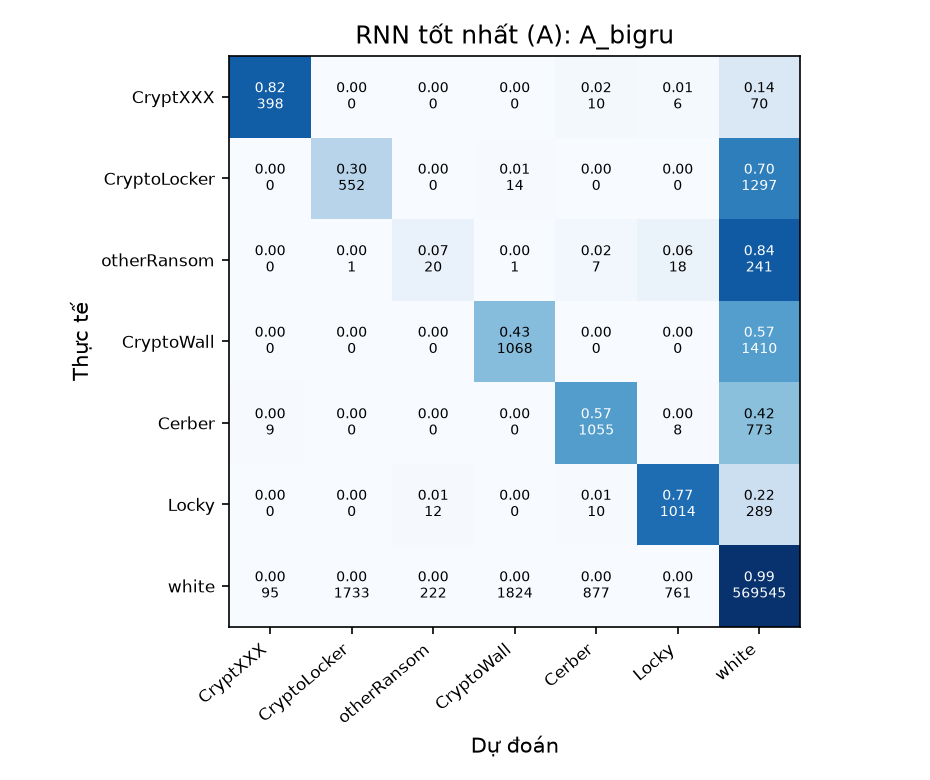
\includegraphics[width=\linewidth]{cm_A_random_A_bigru.png}\caption{RNN tốt nhất (A)}\end{subfigure}
\begin{subfigure}{0.32\linewidth}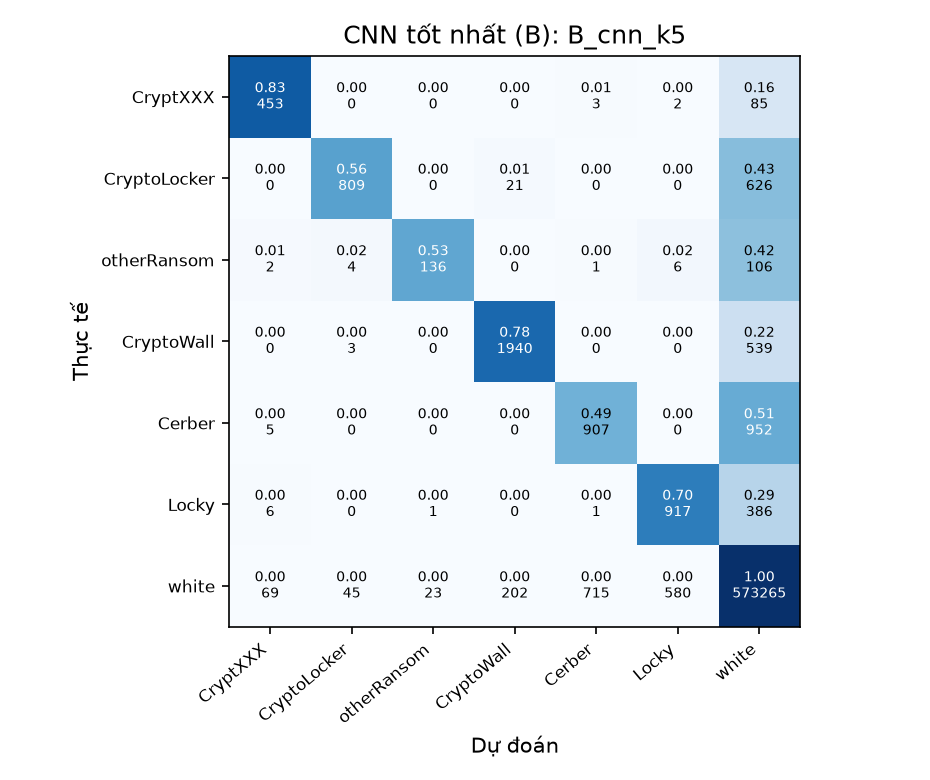
\includegraphics[width=\linewidth]{cm_B_group_B_cnn_k5.png}\caption{CNN tốt nhất (B)}\end{subfigure}
\begin{subfigure}{0.32\linewidth}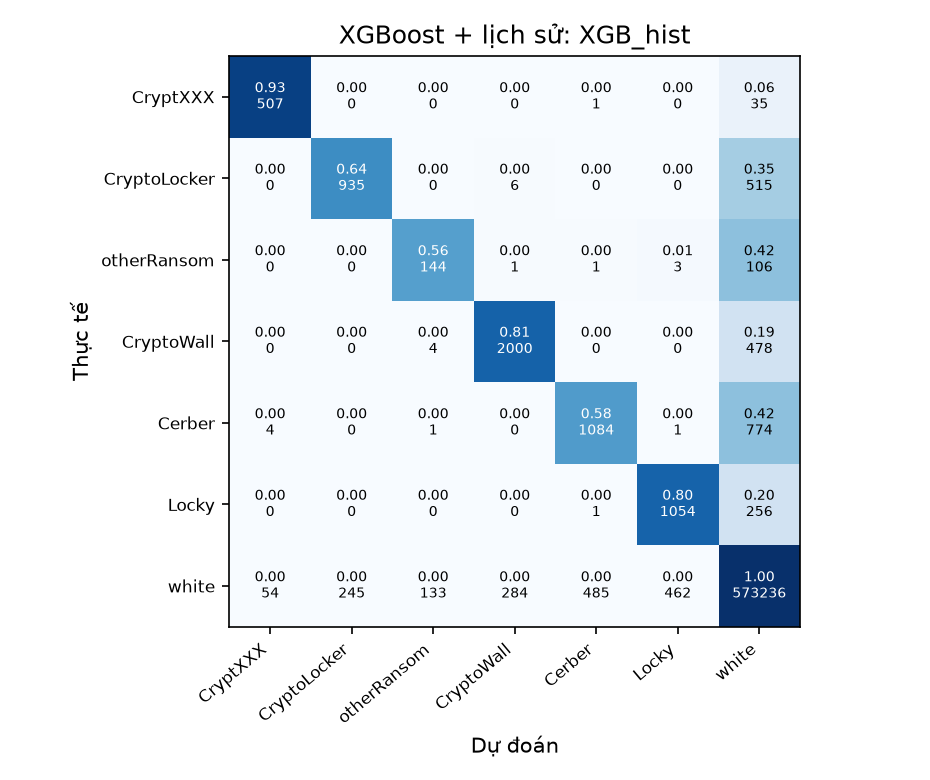
\includegraphics[width=\linewidth]{cm_baseline_group_XGB_hist.png}\caption{XGBoost + lịch sử}\end{subfigure}
\caption{Ma trận nhầm lẫn trên tập test (chuẩn hoá theo hàng = recall từng lớp). Các ma trận khác nằm trong thư mục
\code{outputs/final/figures/} và notebook.}\label{fig:cm}
\end{figure}

\begin{itemize}
\item Lịch sử địa chỉ cải thiện mạnh các họ \textbf{tái sử dụng địa chỉ}: CryptoLocker 0,26 $\to$ 0,70, CryptoWall 0,38 $\to$ 0,84,
  otherRansom 0,08 $\to$ 0,66 (CNN-B; ở lớp này CNN-B còn vượt XGBoost-lịch sử 0,536).
\item Các họ \textbf{dùng địa chỉ mới mỗi lần} (Cerber, Locky: 99\% dòng là lần đầu xuất hiện) không được lợi gì từ lịch sử;
  ở đây XGBoost hơn mạng nơ-ron (Cerber 0,63 so với 0,52--0,56; Locky 0,745 so với 0,65--0,67).
\item Ma trận nhầm lẫn cho thấy lỗi \textbf{gần như hoàn toàn là nhầm giữa ransomware và white}; nhầm giữa các họ ransomware với
  nhau rất hiếm (55 trên 7.911 dòng ransomware với \code{B\_cnn\_k5}). Khó khăn của bài toán là \emph{phát hiện}, không phải
  \emph{phân biệt họ}.
\end{itemize}

\paragraph{Phân tích dự đoán sai (\code{B\_cnn\_k5}, chia theo địa chỉ).} Mô hình bỏ sót 2.694/7.911 dòng ransomware (34\%), trong
đó 78\% là địa chỉ xuất hiện lần đầu; 82\% trong 1.634 báo động nhầm cũng rơi vào địa chỉ lần đầu. Tách theo họ: với CryptoLocker,
CryptoWall và otherRansom, recall trên các dòng \emph{lặp lại} là 0,69/0,92/0,72 nhưng trên các dòng \emph{lần đầu} gần bằng 0 ---
mạng nơ-ron gần như chỉ nhận ra các họ này qua lịch sử, trong khi XGBoost-lịch sử vẫn bắt được 26\%/11\%/11\% dòng lần đầu nhờ đặc
trưng của chính giao dịch. Notebook (mục 10) liệt kê các dòng sai với độ tin cậy cao nhất và ví dụ chuỗi lịch sử tương ứng.

\subsection{Tốc độ huấn luyện}

Thời gian/epoch trong các bảng trên đo khi 6--8 tiến trình huấn luyện chạy song song trên cùng GPU, nên chỉ mang tính tham khảo.
Bảng~\ref{tab:bench} đo lại \emph{riêng từng mô hình} trên GPU rảnh.

\IfFileExists{\tabdir/tab_bench.tex}{\input{\tabdir/tab_bench}}{\textit{(Bảng đo tốc độ sẽ được sinh bởi \code{final/benchmark.py}.)}}

\begin{itemize}
\item \textbf{MLP nhanh nhất} (0,29--0,33 s/epoch): không có chiều chuỗi.
\item Ở biểu diễn A (chuỗi chỉ 11 bước, độ dài cố định), RNN 1 tầng và CNN 2 lớp có tốc độ \emph{gần như nhau}
  (0,39--0,43 s/epoch): cuDNN tối ưu RNN rất tốt cho chuỗi ngắn, còn chi phí BatchNorm/Dropout làm CNN chậm thêm (0,55 s).
  Thêm tầng làm chậm cả hai (LSTM 2 tầng 0,65 s, CNN 3 lớp 0,73 s).
\item Ở biểu diễn B (16 bước, độ dài thay đổi), \textbf{CNN nhanh hơn RNN} $\approx$25\% (0,68 so với 0,89--0,92 s/epoch):
  tích chập tính song song trên mọi vị trí, còn RNN phải tính tuần tự và xử lý \code{pack\_padded\_sequence}. Bi-GRU chậm nhất
  (2,14 s/epoch, gấp 2,4 lần GRU một chiều) mà không tốt hơn.
\item \textbf{GRU ít tham số hơn LSTM} (3 cổng so với 4: 22.439 so với 27.687 tham số ở cấu hình gốc A) và nhanh hơn một chút
  (0,39 so với 0,41 s; 0,53 so với 0,65 s khi 2 tầng).
\item Như vậy ở biểu diễn B, CNN vừa \textbf{nhanh hơn} vừa \textbf{tốt hơn} RNN.
\end{itemize}

\subsection{Trả lời các câu hỏi của đề}

\begin{itemize}
\item \textbf{Mô hình tốt nhất?} Trong các mạng nơ-ron: \code{B\_cnn\_k5} (CNN 1 chiều trên lịch sử địa chỉ, macro F1 0,742).
  Trên toàn bộ đồ án: XGBoost với đặc trưng lịch sử tổng hợp (0,767). Với cùng thông tin một dòng (biểu diễn A), XGBoost Bài 1
  (0,575) tốt hơn mọi RNN/CNN ($\le$0,54).
\item \textbf{Vì sao?} Yếu tố quyết định là \emph{thông tin đầu vào}, không phải loại mạng: thêm lịch sử địa chỉ tăng
  $\approx$0,2 macro F1, còn mọi thay đổi kiến trúc trong cùng một biểu diễn chỉ thay đổi $\le$0,03. CNN tốt hơn RNN một chút trên B vì
  mẫu ``nhận tiền lặp lại vài ngày liên tiếp'' là mẫu \emph{cục bộ}, đúng điểm mạnh của tích chập; XGBoost tốt nhất vì phần lớn
  dòng test không có lịch sử và ở đó mô hình cây dùng đặc trưng dạng bảng hiệu quả hơn.
\item \textbf{Mô hình nhanh nhất?} MLP (Bảng~\ref{tab:bench}). Trong các mô hình chuỗi: ở A, GRU/LSTM 1 tầng và CNN đơn giản
  ngang nhau ($\approx$0,4 s/epoch); ở B, CNN nhanh hơn RNN $\approx$25\%.
\item \textbf{Mô hình ổn định nhất?} Độ lệch chuẩn qua 3 seed của các cấu hình đều nhỏ (0,001--0,008; riêng \code{B\_gru\_cnt} 0,015), nhỏ hơn nhiều so với
  khoảng cách A--B. CNN có BN + Dropout trên B cho đường validation mượt và khoảng cách train--val nhỏ nhất (mục~\ref{sec:analysis}).
\item \textbf{Kết quả có hợp lý không?} Có. Accuracy luôn $>$98\% nhưng vô nghĩa (đoán toàn \code{white} đã đạt 98,6\%), nên
  macro F1 được dùng làm độ đo chính. Lớp \code{white} luôn có F1 $\approx$0,99; các họ có nhiều địa chỉ lặp lại được cải thiện mạnh
  nhờ lịch sử, các họ dùng địa chỉ một lần thì không --- đúng với phân tích dữ liệu ở mục 2. Cách chia theo địa chỉ đảm bảo kết
  quả của B không đến từ việc ``nhớ'' địa chỉ đã thấy khi huấn luyện.
\end{itemize}

\section{Phân tích overfitting / underfitting}\label{sec:analysis}

\paragraph{Cách đọc.} Các đường cong dưới đây vẽ loss (cross-entropy) và macro F1 theo epoch trên tập train (đã undersample) và
\code{val\_us} (validation undersample \emph{cùng tỉ lệ}), nên hai đường so sánh trực tiếp được. Chấm tròn là epoch được early
stopping giữ lại. Lưu ý: số liệu train là trung bình \emph{trong lúc huấn luyện} (dropout đang bật, trọng số thay đổi trong epoch),
nên với mô hình có dropout, F1 train có thể thấp hơn F1 validation. Bảng~\ref{tab:gap} tóm tắt các dấu hiệu chính.

\input{\tabdir/tab_gap}

\begin{figure}[H]\centering
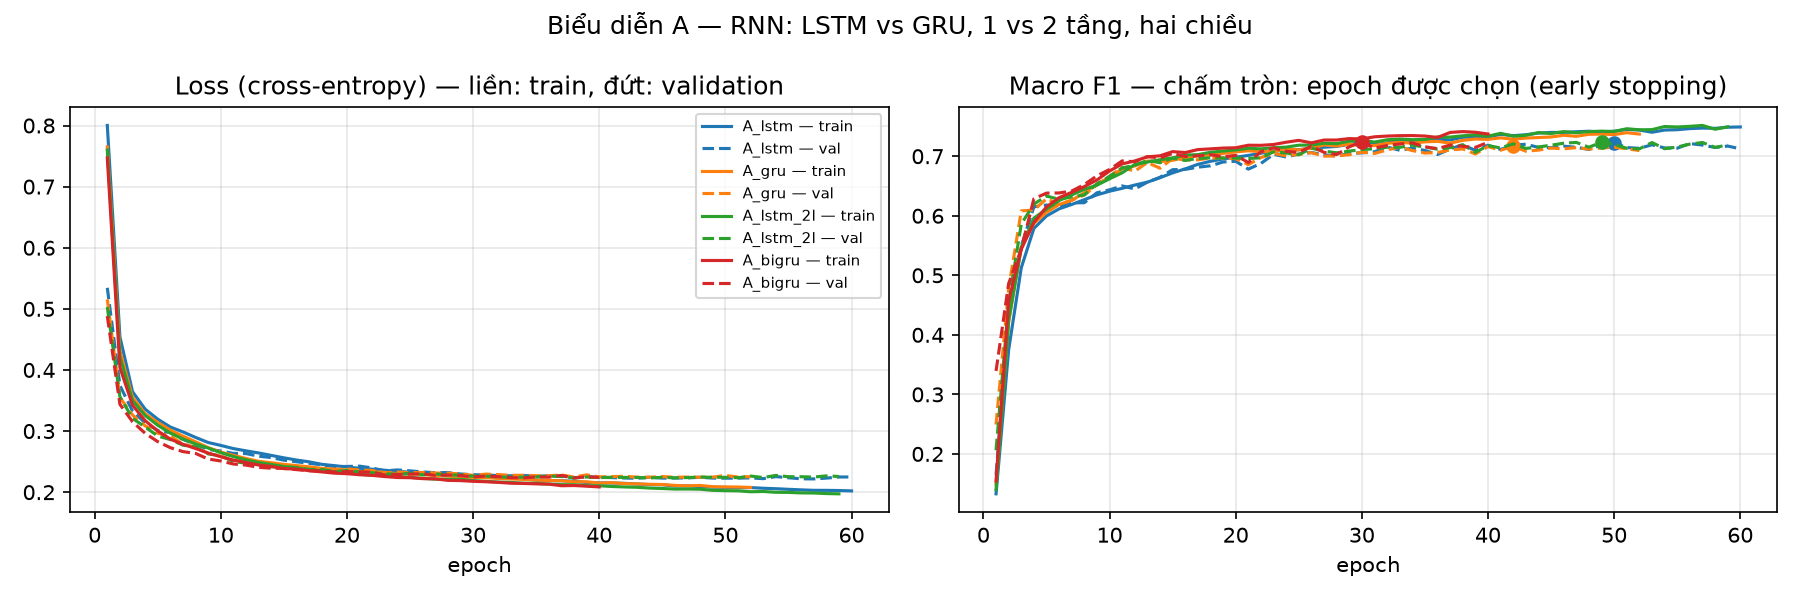
\includegraphics[width=\linewidth]{curves_A_rnn.png}
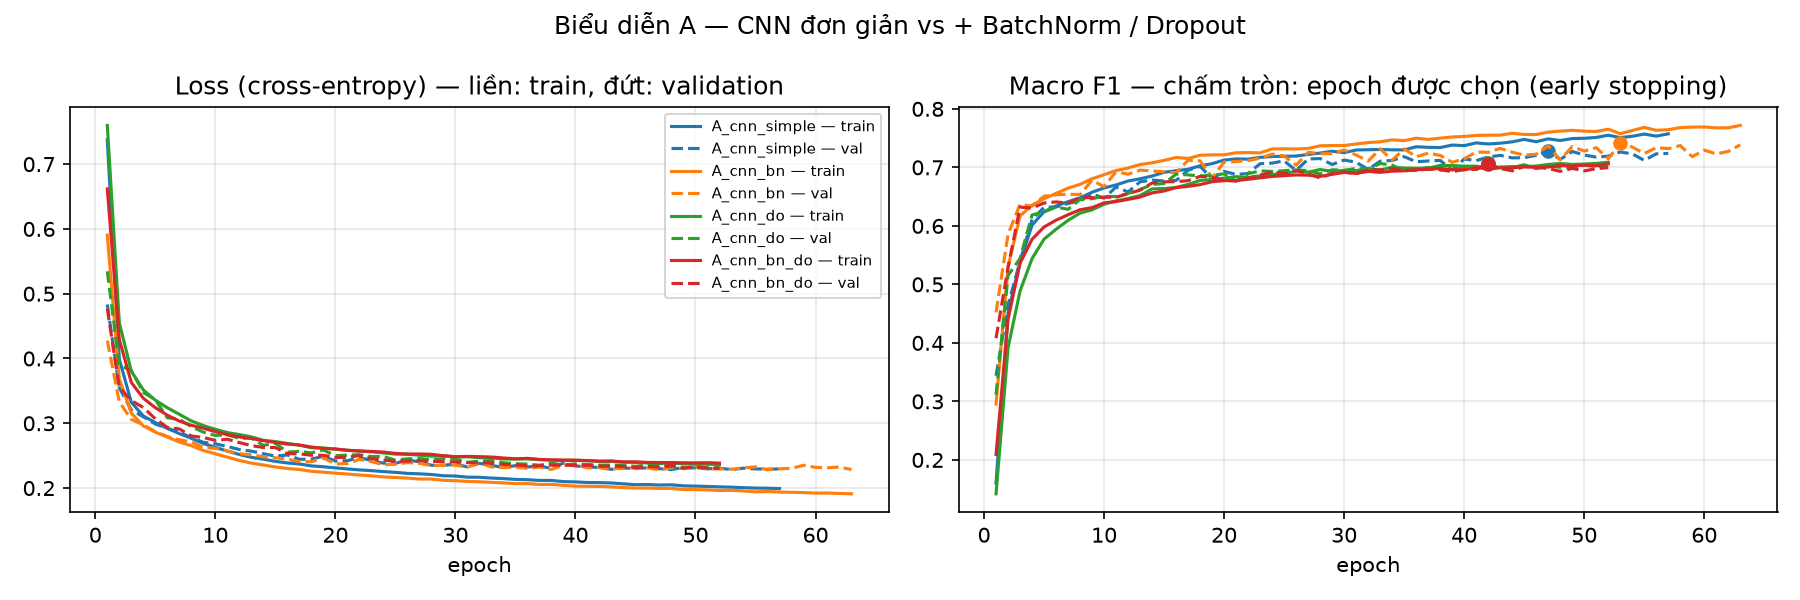
\includegraphics[width=\linewidth]{curves_A_cnn.png}
\caption{Biểu diễn A: RNN (trên) và CNN đơn giản / + BatchNorm / + Dropout (dưới).}\label{fig:curves_A}
\end{figure}

\subsection{Biểu diễn A: giới hạn bởi thông tin, không phải bởi năng lực mô hình}
\begin{itemize}
\item Khoảng cách train--val rất nhỏ ($\le$0,02 macro F1; loss 0,20 so với 0,23) ở mọi cấu hình, và \textbf{tăng năng lực mô hình}
  (2 tầng, 128 units, hai chiều, 3 lớp conv, gấp đôi filters) \textbf{không cải thiện} validation. Đây không phải overfitting, cũng
  không phải underfitting do mô hình quá nhỏ: một dòng đơn lẻ không chứa đủ thông tin để tách ransomware khỏi white (sai số
  không giảm được --- \emph{irreducible error}). XGBoost trên cùng thông tin cũng chỉ đạt 0,575.
\item \textbf{Overfit nhẹ}: \code{A\_gru\_nodrop} và \code{A\_cnn\_bn} có F1 train cao nhất (0,77) và val loss đạt cực tiểu sớm hơn
  epoch tốt nhất (51 so với 63; 47 so với 53) rồi tăng lại (0,232 và 0,229 ở epoch cuối) trong khi train loss tiếp tục giảm --- dấu
  hiệu kinh điển của overfitting. Early stopping dừng kịp; trên test, mức overfit này gần như không gây hại.
\item \textbf{Underfit}:
  \begin{itemize}
  \item \code{A\_cnn\_do}, \code{A\_cnn\_bn\_do}, \code{A\_mlp}: F1 train \emph{thấp hơn} validation, cả hai đều thấp hơn bản không
    dropout. Dropout 0,3 với mô hình chỉ $\approx$23 nghìn tham số là điều chuẩn thừa.
  \item \code{A\_gru\_lr3e-4}: learning rate nhỏ $\Rightarrow$ đường cong tăng chậm, epoch tốt nhất là 84, cả train và val đều thấp
    hơn (0,71/0,71). \code{A\_gru\_bs2048}: batch lớn $\Rightarrow$ số bước cập nhật/epoch giảm 4 lần, epoch tốt nhất 98/100 ---
    \emph{chưa hội tụ} khi hết ngân sách epoch (Hình~\ref{fig:curves_reg}).
  \end{itemize}
\end{itemize}

\begin{figure}[H]\centering
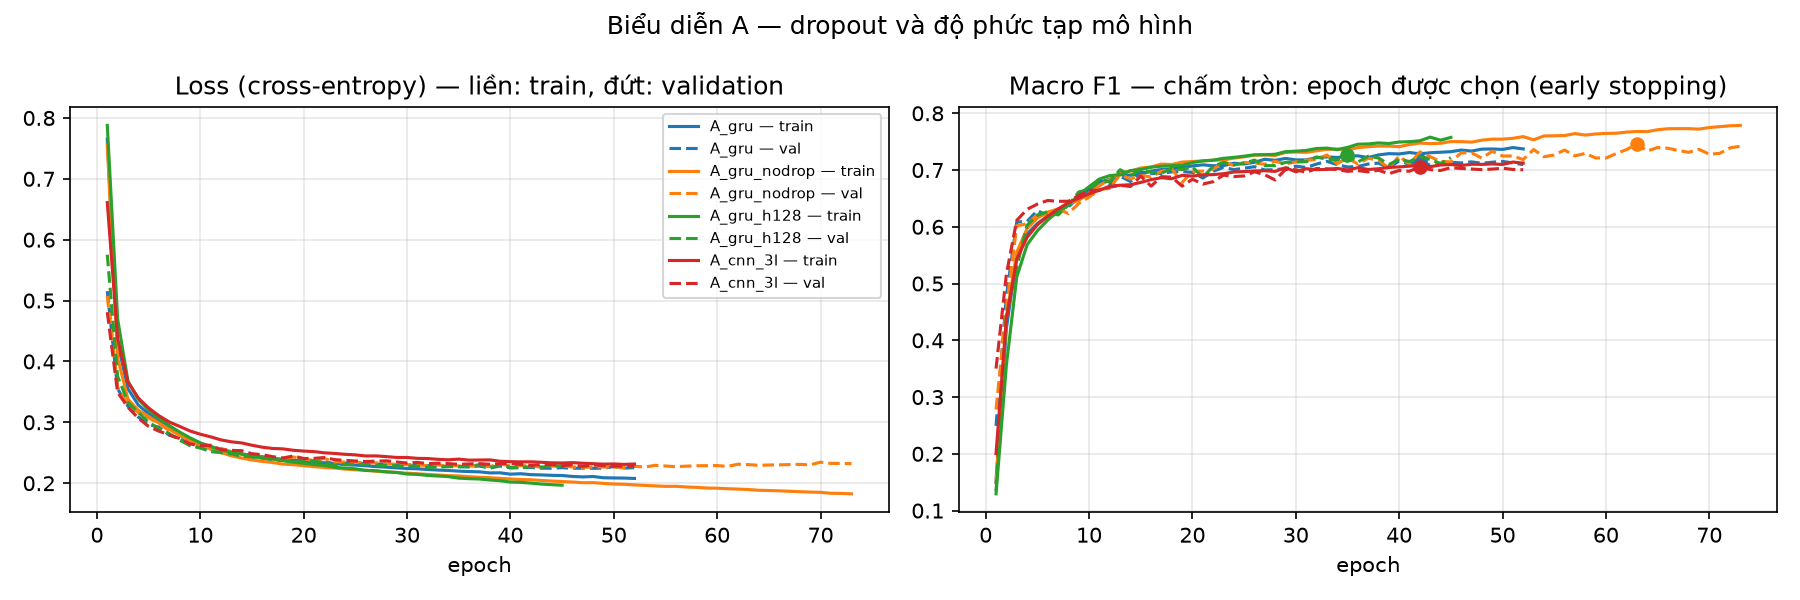
\includegraphics[width=\linewidth]{curves_A_reg.png}
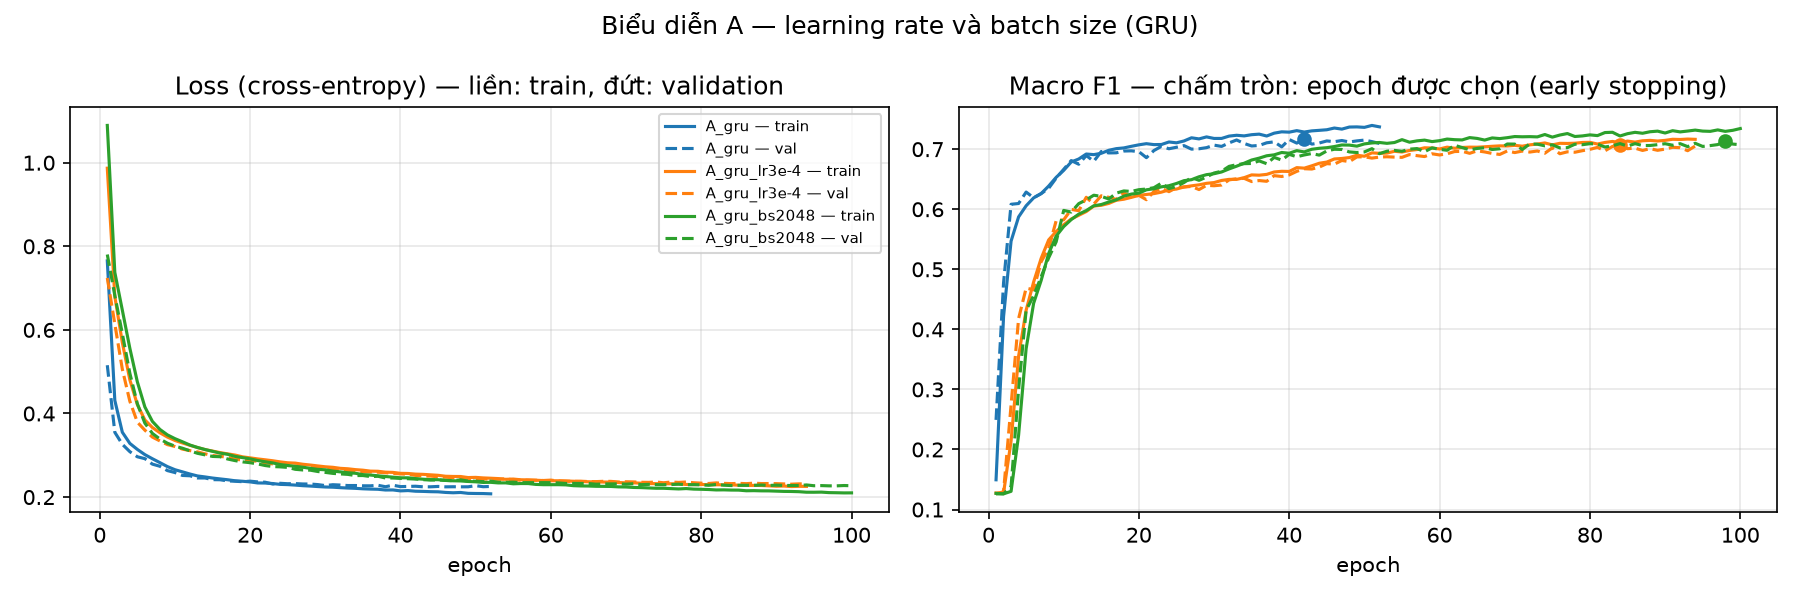
\includegraphics[width=\linewidth]{curves_A_lr.png}
\caption{Biểu diễn A: ảnh hưởng của dropout và độ phức tạp (trên); learning rate và batch size (dưới).}\label{fig:curves_reg}
\end{figure}

\subsection{Biểu diễn B: overfitting rõ hơn và vai trò của điều chuẩn}
\begin{itemize}
\item Với lịch sử, mô hình có nhiều thông tin hơn nên F1 train lên tới 0,91--0,92, và \textbf{khoảng cách train--val lớn hơn hẳn}
  (GRU: 0,911 so với 0,855; val loss 0,169 so với train 0,095 ở epoch cuối). Val loss của \code{B\_gru} đạt cực tiểu ở epoch 22 rồi
  tăng dần, trong khi val F1 vẫn đi ngang/tăng nhẹ đến epoch 53: mô hình tiếp tục \emph{tự tin quá mức} vào các dự đoán sai
  (loss tăng) dù số dự đoán đúng không giảm (F1 không giảm). Vì đề bài đánh giá bằng F1, early stopping theo F1 thay vì loss
  là lựa chọn hợp lý; trọng số lớp $w$ hiệu chỉnh sau cũng bù một phần cho xác suất bị lệch.
\item Nguyên nhân overfit dễ hơn: các dòng của cùng một địa chỉ có lịch sử chồng lấp nhau, nên số mẫu ``độc lập'' thực sự ít hơn
  nhiều so với 126 nghìn dòng (trong toàn bộ dữ liệu, 3.403 địa chỉ CryptoWall/CryptoLocker tạo ra 21.705 dòng, trong khi 9.223 dòng Cerber đến từ 9.177 địa chỉ); mô hình có thể học thuộc
  mẫu riêng của từng địa chỉ trong tập train.
\item \textbf{CNN không điều chuẩn} (\code{B\_cnn\_simple}) overfit nhanh nhất: epoch tốt nhất là 12, chênh F1 tăng từ 0,036 lên
  0,071 ở epoch cuối, test chỉ 0,686. \textbf{Thêm BatchNorm + Dropout} (\code{B\_cnn\_bn\_do}): train/val loss gần trùng nhau
  (0,131/0,136), chênh F1 0,016 --- tổng quát hoá tốt nhất --- và test tăng lên 0,724. Đây là điểm khác so với biểu diễn A:
  \emph{điều chuẩn chỉ có ích khi mô hình thực sự có xu hướng overfit}.
\item GRU 2 tầng (dropout giữa các tầng) có khoảng cách nhỏ hơn GRU 1 tầng (0,034 so với 0,056) và tốt hơn trên test --- dropout
  giữa tầng đóng vai trò điều chuẩn. L=32 overfit sớm hơn (dừng ở epoch 26).
\item \code{B\_mlp} (chỉ bước hiện tại) gần như không overfit nhưng cả train và val đều thấp (0,87/0,85): \emph{underfit} do
  thiếu thông tin lịch sử, không phải do mô hình nhỏ.
\end{itemize}

\begin{figure}[H]\centering
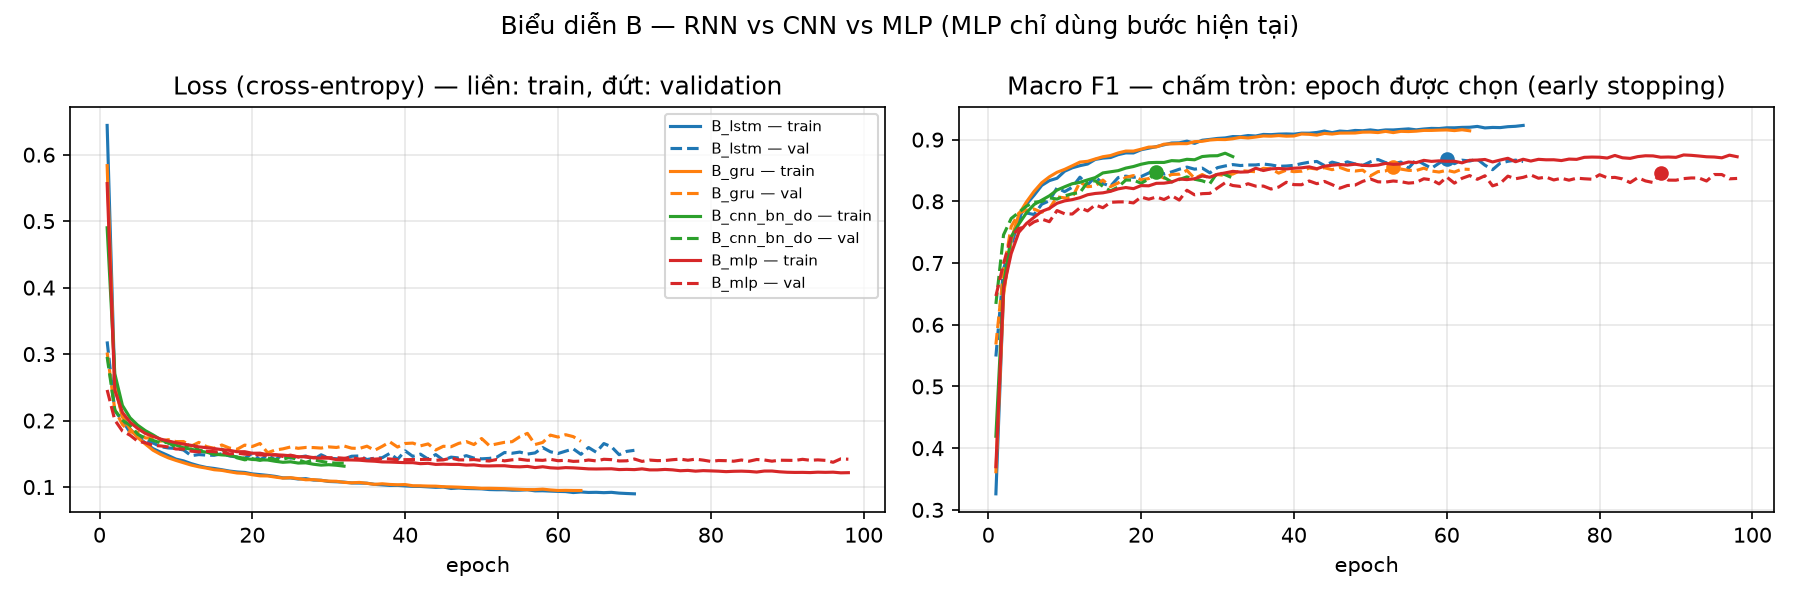
\includegraphics[width=\linewidth]{curves_B.png}
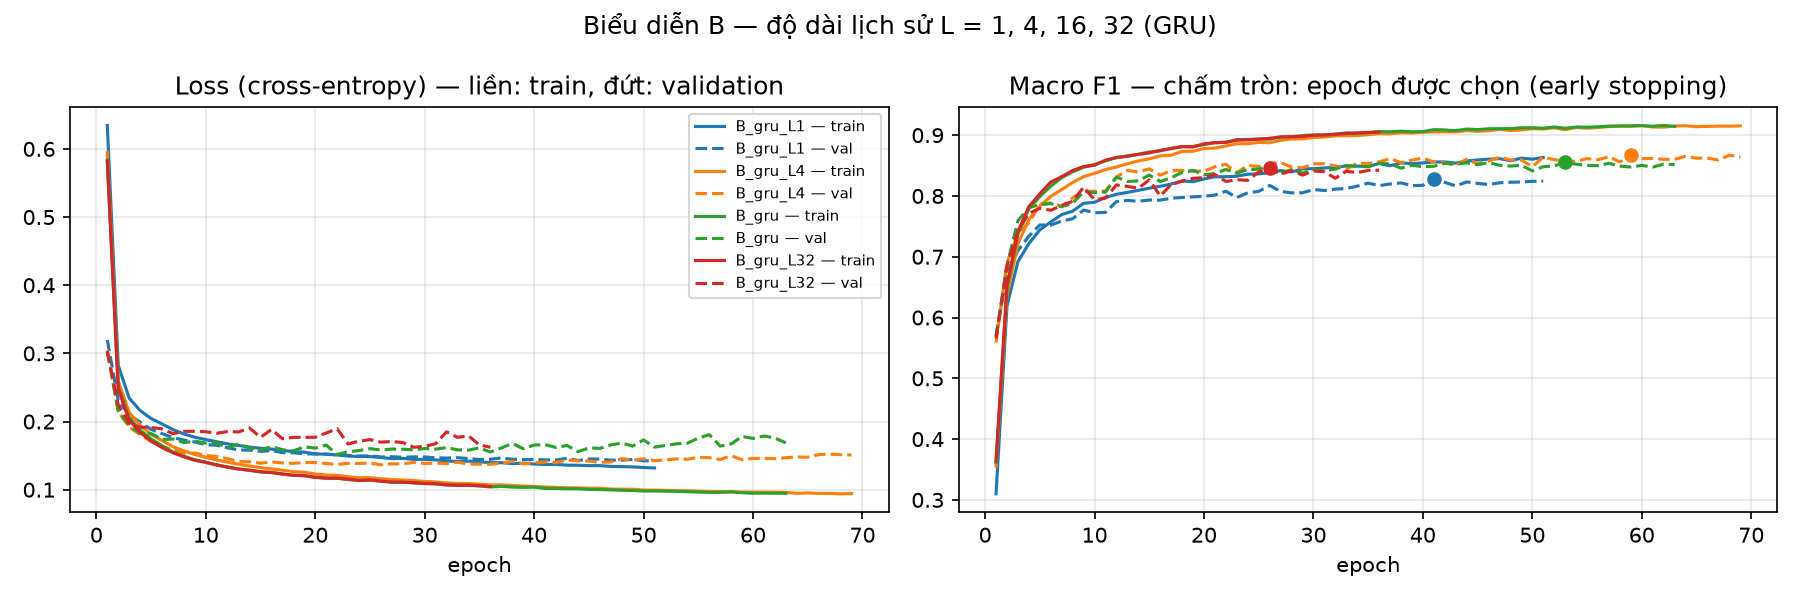
\includegraphics[width=\linewidth]{curves_B_len.png}
\caption{Biểu diễn B: RNN vs CNN vs MLP chỉ dùng bước hiện tại (trên); GRU với độ dài lịch sử L = 1, 4, 16, 32 (dưới).}
\label{fig:curves_B}
\end{figure}

\subsection{Biện pháp đã áp dụng và đề xuất}
\begin{itemize}
\item \textbf{Đã áp dụng}: early stopping (patience 10, khôi phục trọng số tốt nhất) cho mọi mô hình; Dropout ở đầu phân loại và
  giữa các tầng RNN; BatchNorm và Dropout cho CNN; cắt gradient; undersampling + hiệu chỉnh trọng số lớp trên validation.
\item \textbf{Với overfit (biểu diễn B)}: weight decay / L2 (chưa thử --- \code{weight\_decay=0}); giảm số lần xuất hiện được dùng
  của các địa chỉ có rất nhiều dòng (để mỗi địa chỉ đóng góp cân bằng hơn); làm nhiễu lịch sử (bỏ ngẫu nhiên một số bước --- một
  dạng tăng cường dữ liệu cho chuỗi); label smoothing để giảm hiện tượng tự tin quá mức.
\item \textbf{Với underfit}: tăng learning rate hoặc dùng lịch giảm learning rate (cosine/one-cycle) thay vì lr nhỏ cố định; khi dùng
  batch lớn thì tăng lr tương ứng hoặc tăng ngân sách epoch; giảm dropout cho mô hình nhỏ. Với biểu diễn A, cách duy nhất để vượt giới
  hạn là \emph{thêm thông tin} (như biểu diễn B), không phải mô hình lớn hơn.
\end{itemize}

\section{Hạn chế và hướng phát triển}\label{sec:limits}

\subsection{Hạn chế}
\begin{itemize}
\item \textbf{Dữ liệu là dạng bảng, không phải chuỗi tự nhiên.} Biểu diễn A tạo ``chuỗi'' bằng cách xếp 11 đặc trưng theo một thứ
  tự tuỳ ý; RNN/CNN không có lợi thế nào so với MLP và thua mô hình cây. Biểu diễn B là chuỗi thật (theo thời gian) nhưng chỉ có ích
  cho địa chỉ được dùng lại --- 90\% dòng test là địa chỉ xuất hiện lần đầu, chuỗi chỉ dài 1.
\item \textbf{Lớp \code{white} được lấy mẫu} (khoảng 1.000 dòng/ngày trong dữ liệu gốc), nên ``lịch sử'' của một địa chỉ white bị
  thưa hơn thực tế, và đặc trưng ``số lần đã xuất hiện'' có thể phân biệt hai lớp tốt hơn so với khi triển khai thật trên toàn bộ
  chuỗi khối. Kết quả của biểu diễn B có thể lạc quan so với thực tế.
\item \textbf{Nhãn ransomware không đầy đủ}: chỉ các địa chỉ đã được các nghiên cứu trước xác định; nhiều dòng \code{white} có thể là
  ransomware chưa được phát hiện, làm giảm precision quan sát được.
\item \textbf{Hai cách chia khác nhau}: biểu diễn A dùng chia ngẫu nhiên (để so sánh với Bài 1) --- 54,7\% dòng ransomware trong test
  có địa chỉ đã xuất hiện trong train, nên kết quả A có rò rỉ nhẹ qua địa chỉ. Bảng~\ref{tab:group_other} đã kiểm chứng: trên cách chia
  theo địa chỉ, A cho kết quả gần như giống hệt, nên kết luận không thay đổi.
\item \textbf{Ước lượng phương sai còn hạn chế}: chỉ 3 seed cho các cấu hình chính (1 seed cho các biến thể còn lại), và chỉ một cách
  chia dữ liệu (không cross-validation). Khác biệt $<$0,01 giữa các cấu hình không nên coi là có ý nghĩa.
\item \textbf{Early stopping theo \code{val\_us}} (31,6 nghìn dòng, chỉ $\approx$6,6 nghìn dòng ransomware) có nhiễu; nhiều cấu hình A
  cùng seed dừng ở cùng epoch (42) vì dùng chung thứ tự batch, cho thấy chọn epoch phụ thuộc phần nào vào dao động ngẫu nhiên.
\item \textbf{Siêu tham số chưa tối ưu toàn diện}: thay đổi từng yếu tố một so với cấu hình gốc (không tìm kiếm lưới/Bayes);
  không thử recurrent dropout, weight decay, lịch learning rate. Thời gian/epoch trong bảng chính bị ảnh hưởng do chạy song song
  (đã đo lại riêng ở Bảng~\ref{tab:bench}).
\end{itemize}

\subsection{Hướng phát triển}
\begin{itemize}
\item \textbf{Kết hợp hai thế mạnh}: mô hình cây cho đặc trưng của dòng hiện tại và RNN/CNN cho lịch sử --- ví dụ dùng embedding
  lịch sử do CNN-B học được làm đặc trưng đầu vào cho XGBoost, hoặc ensemble xác suất của hai mô hình (XGBoost tốt hơn ở địa chỉ
  mới, CNN-B tốt hơn ở địa chỉ có lịch sử dài --- Bảng~\ref{tab:by_len}).
\item \textbf{Mô hình đồ thị}: ransomware chuyển tiền qua nhiều địa chỉ; cần dữ liệu giao dịch gốc (cạnh giữa các địa chỉ) để dùng
  Graph Neural Network --- giúp cả với địa chỉ dùng một lần như Cerber/Locky.
\item Transformer trên lịch sử địa chỉ (self-attention với mã hoá khoảng cách thời gian); mô hình FT-Transformer [8] cho biểu diễn A.
\item Tối ưu siêu tham số tự động (Optuna), nhiều seed hơn, cross-validation theo địa chỉ, và hiệu chỉnh xác suất (temperature scaling)
  trước khi tìm ngưỡng/trọng số lớp.
\item Đánh giá theo thời gian (train trên các năm trước, test trên năm sau) để mô phỏng triển khai thực tế và kiểm tra khả năng phát hiện
  họ ransomware mới.
\end{itemize}


\section*{Tài liệu tham khảo}
\addcontentsline{toc}{section}{Tài liệu tham khảo}
\begin{enumerate}[label={[\arabic*]}]
\item C.~G. Akcora, Y.~Li, Y.~R. Gel, M.~Kantarcioglu. \emph{BitcoinHeist: Topological Data Analysis for Ransomware Detection on the Bitcoin Blockchain}. IJCAI-PRICAI 2020. Bộ dữ liệu: UCI Machine Learning Repository, \emph{BitcoinHeistRansomwareAddressDataset}.
\item S.~Hochreiter, J.~Schmidhuber. \emph{Long Short-Term Memory}. Neural Computation 9(8), 1997.
\item K.~Cho và cộng sự. \emph{Learning Phrase Representations using RNN Encoder–Decoder for Statistical Machine Translation}. EMNLP 2014 (GRU).
\item Y.~LeCun, Y.~Bengio. \emph{Convolutional Networks for Images, Speech, and Time Series}. The Handbook of Brain Theory and Neural Networks, 1995.
\item S.~Ioffe, C.~Szegedy. \emph{Batch Normalization}. ICML 2015.
\item N.~Srivastava và cộng sự. \emph{Dropout: A Simple Way to Prevent Neural Networks from Overfitting}. JMLR 15, 2014.
\item D.~P. Kingma, J.~Ba. \emph{Adam: A Method for Stochastic Optimization}. ICLR 2015.
\item Y.~Gorishniy và cộng sự. \emph{Revisiting Deep Learning Models for Tabular Data}. NeurIPS 2021 (ý tưởng mã hoá mỗi đặc trưng thành một token).
\item L.~Grinsztajn, E.~Oyallon, G.~Varoquaux. \emph{Why do tree-based models still outperform deep learning on tabular data?} NeurIPS 2022 Datasets and Benchmarks.
\item T.~Chen, C.~Guestrin. \emph{XGBoost: A Scalable Tree Boosting System}. KDD 2016.
\item Thư viện: PyTorch 2.11, scikit-learn 1.x, XGBoost, pandas, NumPy, Matplotlib.
\end{enumerate}

\appendix
\section{Mã nguồn và cách chạy lại}\label{app:code}

\paragraph{Cấu trúc.}
\begin{itemize}
\item \code{final/data.py} --- đọc dữ liệu, tạo nhãn 7 lớp và đặc trưng, chia ngẫu nhiên / theo địa chỉ, undersampling, dựng lịch sử
  địa chỉ (biểu diễn B), chuẩn hoá (chỉ tính trên train).
\item \code{final/models.py} --- \code{FeatureTokenizer} (biểu diễn A), \code{RNNNet} (LSTM/GRU, 1--2 tầng, một/hai chiều,
  last/mean/attention, \code{pack\_padded\_sequence}), \code{CNNNet} (Conv1D, BN, Dropout, Max/Avg pooling, Flatten/GAP/GMP có mặt nạ),
  \code{MLPNet}.
\item \code{final/configs.py} --- toàn bộ cấu hình thực nghiệm (tên, kiến trúc, siêu tham số).
\item \code{final/train.py} --- huấn luyện với early stopping, ghi lịch sử từng epoch, hiệu chỉnh trọng số lớp trên validation,
  đánh giá test; lưu \code{history.json}, \code{result.json}, \code{model.pt}, \code{pred\_test.npy} vào
  \code{outputs/final/<biểu diễn>\_<cách chia>/<cấu hình>/}.
\item \code{final/baselines.py} --- XGBoost (GPU) trên hai cách chia với 3 mức thông tin lịch sử.
\item \code{final/benchmark.py} --- đo tốc độ huấn luyện từng mô hình khi chạy riêng.
\item \code{final/report.py} --- tổng hợp kết quả thành các bảng LaTeX/CSV (\code{outputs/final/tables/}) và hình
  (\code{outputs/final/figures/}) dùng trong báo cáo.
\item \code{final\_project.ipynb} --- notebook trình bày đầu--cuối: thống kê dữ liệu, minh hoạ hai biểu diễn, in kiến trúc, bảng kết quả,
  đường cong huấn luyện, ma trận nhầm lẫn, dự đoán mẫu và phân tích lỗi. Mặc định notebook \emph{nạp kết quả đã huấn luyện};
  đặt \code{RETRAIN = True} để huấn luyện lại một số cấu hình tiêu biểu ngay trong notebook.
\end{itemize}

\paragraph{Cách chạy.} Cần Python 3.12, các thư viện trong \code{requirements.txt} (thêm PyTorch có CUDA nếu dùng GPU) và tệp
\code{BitcoinHeistData.csv} ở thư mục gốc. Siêu tham số XGBoost được đọc từ \code{exp\_out/best\_params.json} (kết quả tinh chỉnh
của Bài 1).
{\footnotesize
\begin{verbatim}
pip install -r requirements.txt
python -m final.train --rep A            # mọi cấu hình A, chia ngẫu nhiên
python -m final.train --rep B            # mọi cấu hình B, chia theo địa chỉ
python -m final.train --rep A --split group --only A_gru+A_lstm+A_mlp+A_cnn_bn_do
python -m final.train --rep B --seeds 43+44 --only B_gru+B_cnn_bn_do  # seed khác
python -m final.baselines                # XGBoost
python -m final.benchmark                # đo tốc độ (khi GPU rảnh)
python -m final.report                   # bảng + hình
cd report && latexmk -xelatex main.tex   # biên dịch báo cáo
\end{verbatim}
}
Có thể chạy nhiều tiến trình \code{final.train} song song với cùng tham số: mỗi tiến trình ``nhận'' một cấu hình chưa chạy
(qua một tệp khoá) nên không chạy trùng. Thời gian: $\approx$0,5--2,5 phút/cấu hình A và 0,5--7 phút/cấu hình B trên GPU RTX PRO 4000 (khi chạy song song).

\paragraph{Tái lập.} Chia dữ liệu và undersampling luôn dùng \code{random\_state=42}; seed huấn luyện (42, 43, 44) cố định khởi tạo trọng số và thứ tự batch. Do một số phép
toán cuDNN không tất định, chạy lại có thể khác ở chữ số thập phân thứ 3 --- nhỏ hơn độ dao động giữa các seed.


\end{document}
